\chapter{发现}[Findings]

本章主要对前一章的实验数据进行统计和经验性总结。并试图通过对已有的实验数据总结回答以下问题:适合自动驾驶系统测试用例生成的对抗生成网络和图像风格转换技术的路况图像实际合成效果如何?各个模型的实际训练效率如何?哪个或哪几个深度学习模型总体是最适合自动驾驶系统测试用例的自动生成?

\section{实验数据统计}[Experiments Statistics]

\textbf{训练时长.}\quad 在将我们找到的能够实现驾驶场景图片转换功能的模型基于Udacity自动驾驶数据集\cite{udacity_dataset}和已有的从Youtube上爬取的数据集进行图像转换实验,且得到各个模型是合成图数据后,我们首先统计的指标是各个模型的\textbf{训练时长}。所有模型的训练平台硬件环境都一致:Ubuntu 16.04 LTS操作系统,8核GeForce GTX 1080ti GPU。训练时长的工具使用的是GNU开源工具\textit{time},统计数据如下表\ref{table:time}:

\begin{table}[h]
    \centering
    \begin{tabular}{p{3cm}|rrr}
        \hline
        \mthead{模型名称} & \mthead{real} & \mthead{user} & \mthead{sys} \\
        \hline
        MUNIT & 3743m77.651s & 4927m93.474s & 837m.52.196s \\
        \hline
        CycleGAN & 3154m38.274s & 4081m81.696s & 731m20.894s \\ \hline
        EBGAN & 3811m24.172s & 5021m32.721s & 757m19.141s \\ \hline
        AdaIn Style & 2349m46.212s & 3782m18.764s & 554m26.476s \\ \hline
        Deep Photo Style Transfer & \multicolumn{3}{c}{\textit{pre-trained}} \\ \hline
        Fast Photo Style & \multicolumn{3}{c}{\textit{pre-trained}} \\ \hline
        Fast Neural Transfer & \multicolumn{3}{c}{\textit{pre-trained}} \\ \hline
        Texture Nets & \multicolumn{3}{c}{\textit{pre-trained}} \\ \hline
    \end{tabular}
    \caption{模型训练时间统计}
    \label{table:time}
\end{table}
因为图像风格转换技术中,除了Adain Style,其他都是直接使用的文献中给定的pre-trained模型,一般都是VGG网络。在已有的数据中可以看到MUNIT训练用时最长。因此我们建议如果时间不充裕的情况下可以优先考虑使用图像风格转换技术的模型,对于模型风格不同的需求可以通过更换提前训练好的模型网络来实现,而无需想对抗生成网络一样对新数据重新进行一遍整体模型的训练。尽管大部分图像风格转换技术有无需对整体模型进行训练的便利,但我们在实验中发现图像风格转换技术对单张图片的转换时间比训练好的对抗生成网络模型耗时要更长,一般训练好的对抗生成网络模型单张图片合成平均耗时约5秒左右,而我们统计的图像风格转换技术依具体模型不同耗时在1分钟到20分钟。因此如果考虑到实时图形转换,譬如视频实时合成的需求,则对抗生成网络大类的技术是更好的选择。

\textbf{FID.}\quad 我们参考了文献\cite{FID},使用代码\cite{git:fid}计算了8个模型合成图的fid值,下表\ref{table:fid}为最后的结果统计数据: 

\begin{table}[h] 
    \centering
    \begin{tabular}{|l|*{4}{p{2.5cm}|}}
        \hline
        模型 & MUNIT & CycleGAN & EBGAN & AdaIN Style  \\ \hline 
        FID值 & 185.18924 & 275.04948 & 217.82906 & 88.39498  \\ \hline
        模型 & Deep Photo Style & Fast Photo Style & Fast Neural Transfer & Texture Nets \\ \hline
        FID值 & 77.28563 & 139.49777 & 92.61378 & 87.31297 \\ \hline
    \end{tabular}
    \caption{FID值统计表}
    \label{table:fid}
\end{table}

可以对抗生成网络类模型的FID得分普遍比图像风格转换技术的得分要差,根据FID计算的原理以及两者模型类别合成图的特点,我们分析以上原因可能主要是因为图像风格转换技术一般不会对图像的内容结构有较大改变,而对抗生成网络往往会对图像的边界、结构做出较大改动比如下图\ref{fig:gan}为UNIT的典型的合成图片样本。
\begin{figure}[h]
    \centering
    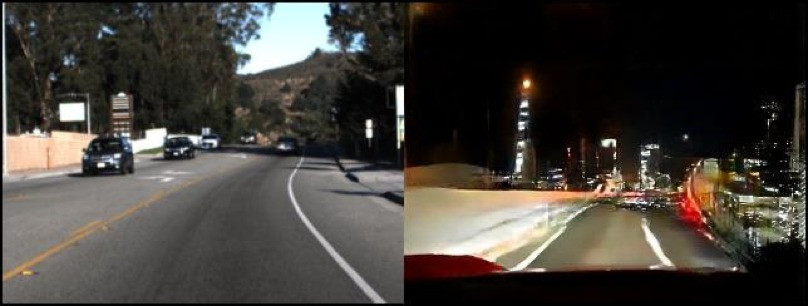
\includegraphics[width=.8\textwidth]{gan_bad}
    \caption{UNIT合成图像样本}
    \label{fig:gan}
\end{figure}
可以看到合成图片中道路和旁边的街景边界已经变得十分模糊,且合成图片与原图像在图像内容上相差也较大。而FID计算的是两者图像间的差异及FID计算过程中自动提取的特征差别,相比之下图像风格转换技术对图像的改动更多的倾向于像素色调,图像内容边界扰动等,所以其在FID得分上可预见性的要普遍优于对抗生成网络。以上也给我们一个启发,如果我们希望合成的图像相对原图像在语义边界、内容上的改动尽可能的要小,则我们推荐采用图像风格转换类模型进行图像合成,反之如果希望合成的图像更多的综合内容图像和风格图像的特点,或者更多的包含风格图像的特点,则对抗生成网络类技术是更好的选择。 

\textbf{方向盘拐角.}\quad 为了测出每个模型最终的合成图对自动驾驶系统的干扰,即合成图的拐角与原图的拐角差,实验中自动驾驶拐角预测模型我们使用了Udacity自动驾驶竞赛中的cg23\cite{cg23}模型。由于模型代码的限制,在输出拐角前还必须对已有的合成图做相应的时间戳标记,这一部分使用了Udacity Driving Reader代码\cite{git:udr}。期间,由于作者提供的最初的实验代码中有大量是基于Udacity自动驾驶竞赛定制的代码,无法很好的移植到我们的实验中,于是在参考了其他代码后我们融合了cg23和该竞赛中其他模型的拐角预测代码,整体模型是基于Tensorflow构造的6层卷积神经网络实现的。得到了所有图片在自动驾驶系统下的方向盘拐角预测值后,为了显示出其与原始图片在自动驾驶系统下的预测拐角值偏差,我们计算了所有单张图与原图拐角差值的平均方差,以此来总体评价合成图对自动驾驶系统的干扰。最终我们使用Python的Matplotlib库将差值数据可视化的绘制在图表上。

图\ref{fig:sad}是MUNIT和CycleGAN最终的拐角偏差数据,完整的模型拐角变差数据见附录拐角数据统计表。
\begin{figure}[!h]
    \subfigure[MUNIT]{
        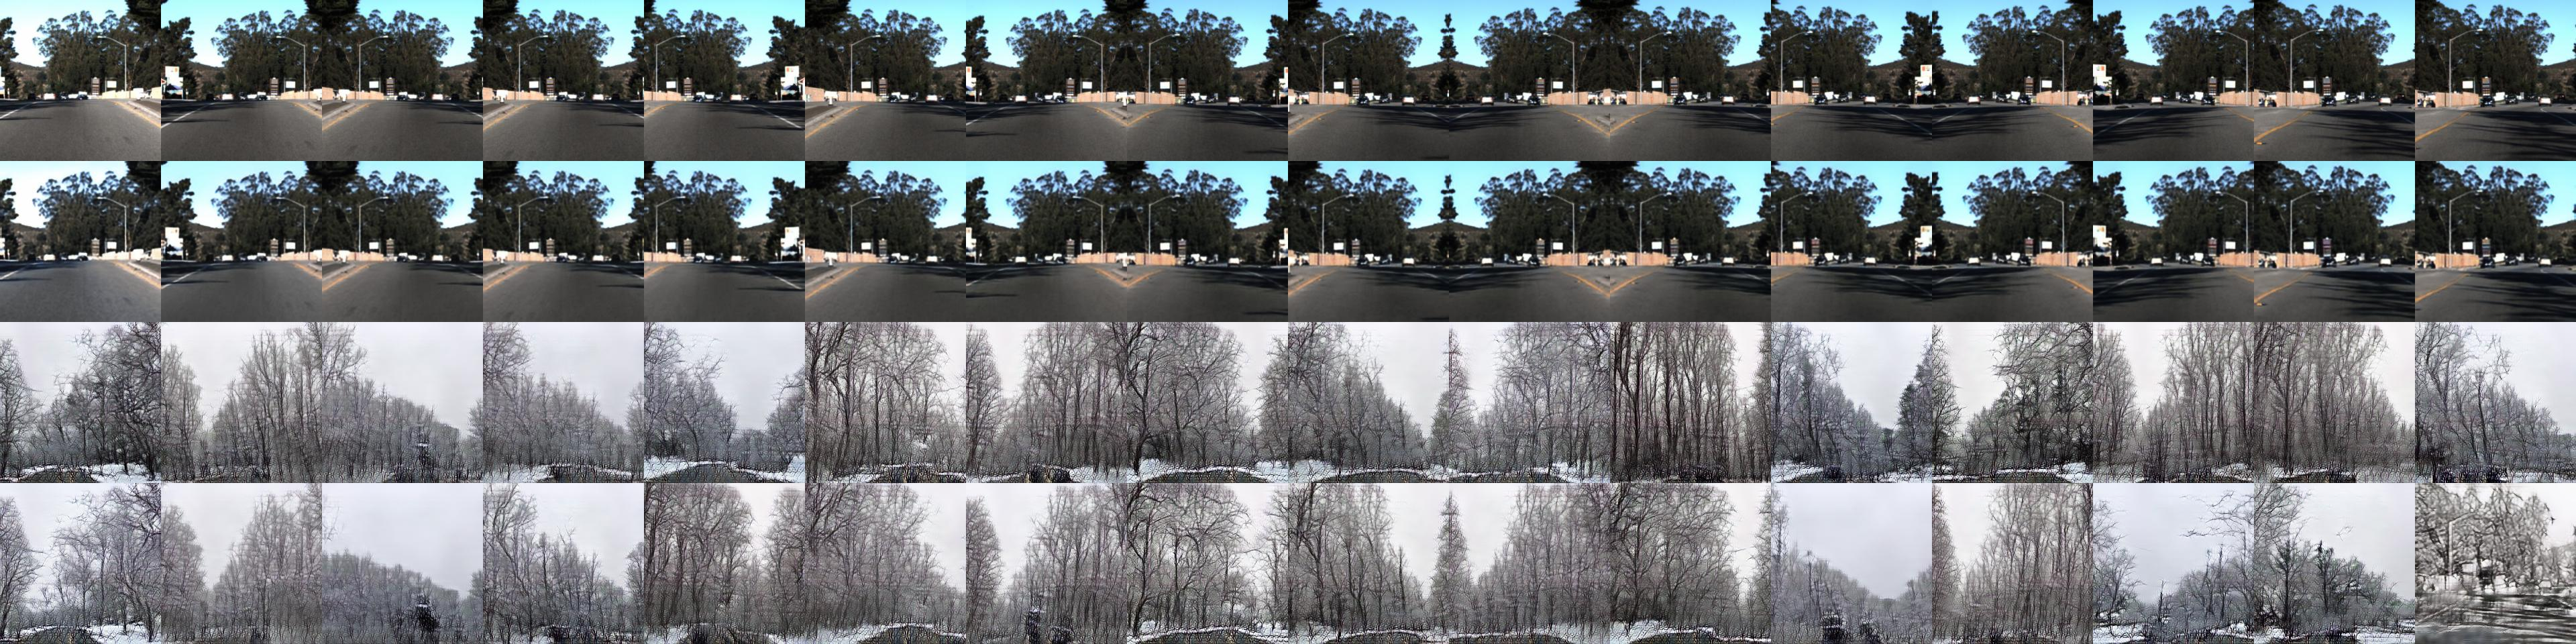
\includegraphics[width=1.5\textwidth, center]{rmse/1} 
    }
    \subfigure[CycleGAN]{
        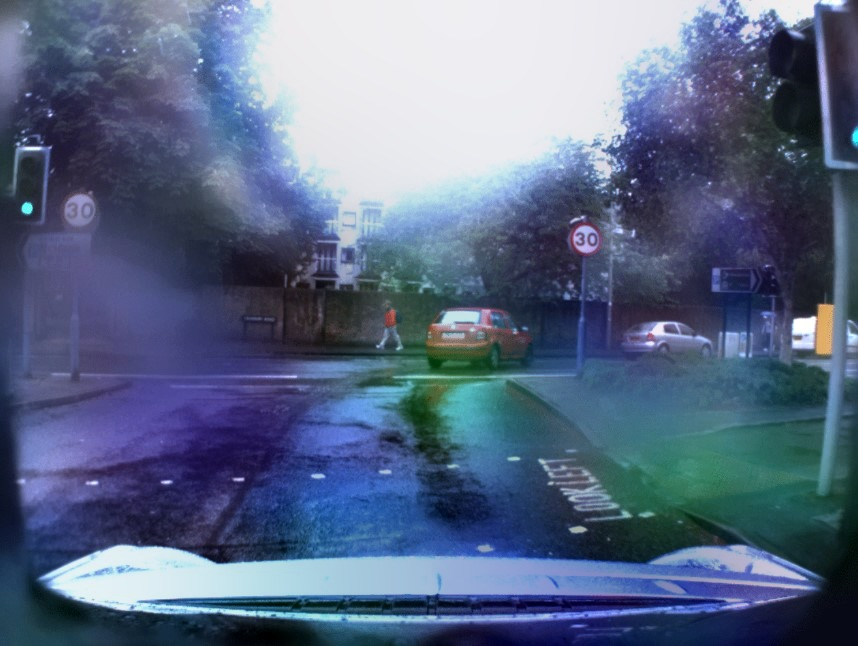
\includegraphics[width=1.5\textwidth, center]{rmse/2} 
    }
    \caption{方向盘拐角差}
    \label{fig:sad}
\end{figure}


图中红色是原图在自动驾驶中的拐角,蓝色是合成图的拐角差,横轴是处于某一时间戳的图片。从数据可以看出对抗生成网络的合成图对自动驾驶系统行为的干扰会比图像风格转换技术合成图造成的干扰大。通过对合成图的进一步分析,我们发现自动驾驶系统对于训练过程中使用了语义分割技术的模型合成图,预测的拐角误差相对较小,比如Fast Photo Style中虽然使用的是提前训练好的vgg19网络,但在进行图像转换前,需要对待转换的图片进行一步语义分割的预处理,这种类型技术转换后的团向与原图内容基本没有太大变化,更多的是再原图基础上对不同像素点进行亮度修改,比如下图\ref{fig:seg}为Fast Photo Style进行语义分割后的合成效果图。相较对抗生成网络,比如UNIT的合成图\ref{fig:gan},合成图像中道路、树木甚至阴影的可以十分清晰的区分开。由于自动驾驶系统模型的训练数据集通常都是真实场景的路况图片,所以对于诸如UNIT合成图像在方向盘拐角预测上效果比图像转换技术合成图效果要相差很多,这也符合我们最终统计的实验数据。

\begin{figure}[h]
    \centering
    \subfigure[语义分割图]{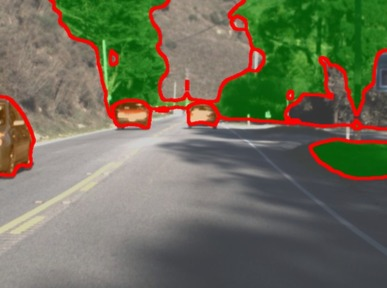
\includegraphics[width=.3\textwidth]{fps_s_1}}
    \subfigure[风格图片]{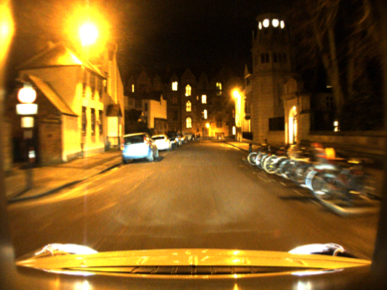
\includegraphics[width=.3\textwidth]{fps_s_3}}
    \subfigure[合成图像]{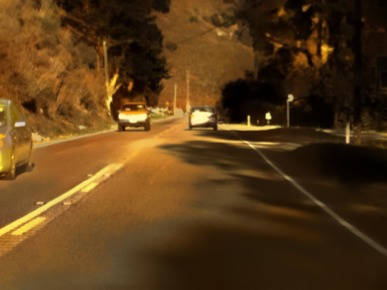
\includegraphics[width=.3\textwidth]{fps_s_2}}
    \caption{语义分割合成图}
    \label{fig:seg}
\end{figure}


\section{实验数据发现总结与展望}[Experiments Findings]

\subsection{发现总结}

在综合了最后的实验数据,我们有以下几点发现:

\textbf{几乎所有能够实现图像转换的深度学习模型最后的合成图像都对模型的训练数据十分敏感},其中MUNIT最为显著,因为该模型给出的范例有基于路况图片进行转换的示例,但其训练集中,内容图片集合与样式数据集中图片的内容十分接近。由于示例汇中使用的是NVIDIA提供的闭源数据,所以我们不能复现其示例中的实验结果,且我们的数据集中内容数据集(Udacity路况图片集)与样式数据集其内容差距比较明显,所以最终的实现效果较示例中的效果要差很多。这点从之前的实验结果样例图中可以很清晰的看出。

因此,我们认为在自动驾驶系统测试用例的自动生成,或者一般性的图像风格转换工作中,如果想要最终获得效果令人满意的合成图,那么无论采用的是对抗生成网络技术还是需要训练模型的图像风格转换技术,训练数据集,即内容图片集和风格图片集至关重要,甚至直接影响了图像的最终合成效果。此外,通过比较我们的实验结果和模型的官方合成效果极其训练数据集,不难看出在进行图像风格转换过程中,内容图像集和风格图像集的图像结果和内容应尽可能的接近,甚至建议在选择图像集前,对内容图像集和风格图像集进行一次FID值计算,以此来量化两者的相近程度。这一点我们也考虑添加到后续研究中,以此来证实内容图像集与风格图像集的相近程度是否与模型的最终合成图成像品质成正比。但从已有的数据中我们对于这个结果还是持肯定态度的。

其次在仔细查看所有模型的最终合成图后我们发现,\textbf{相比图像转换技术,对抗生成网络的合成图片中,会新增有很多样式图片集中特有,而原图像没有的元素}。新出现的元素或物体常常所欲风格图片集中的物体,比如图\ref{fig:new}所示,右边合成图中间出现了本属于风格图像集中的街景物体,从图片整体上来看,合成图的整体图像风格以及图形语义结构似乎更接近于风格图像集了。相较原图,合成图只较完整的保留了道路的图像内容,原图中的车辆树木在合成图中都已经消失了。而图像转换技术合成图片中,典型的如图\ref{fig:new}中下图所示,合成图图像内容上几乎和原图是保持一致不变的,物体的减少和新增的情况很少出现。且图像转换技术合成的图片中,主要针对的是对远图像中像素的颜色通道和明暗值做修改,这跟对抗生成网络类的模型有很大的不同。从这一点上,图像风格转换技术相较对抗生成网络技术更贴近风格转换的功能需求。

\begin{figure}[h]
    \centering
    \subfigure[出现新物体的GAN合成图]{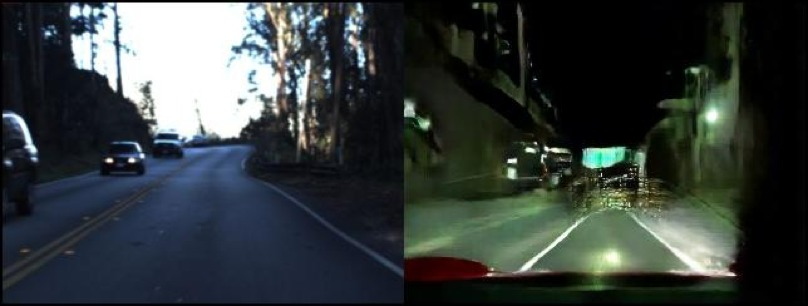
\includegraphics[width=.75\textwidth]{gan_n}}
    \subfigure[典型的图像风格转换合成图]{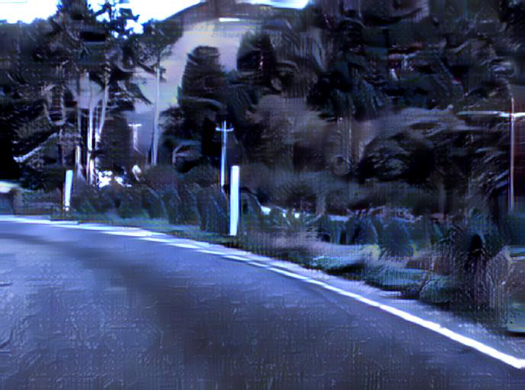
\includegraphics[width=.5\textwidth]{nst_n}}
    \caption{合成图效果对比}
    \label{fig:new}
\end{figure}

在对FID值统计数据的调查中我们发现,原本预想中的图像集的FID值与自动驾驶系统行为干扰的强相关并没有出现。比如EBGAN的合成图FID值为217.82906要高于MUNIT合成图的185.18924,但其方向盘拐角差方差要比MUNIT小很多,即对自动驾驶系统的干扰要小很多。但是利用图像转换技术合层的图片,要比使用对抗生成网络模型合成的图片,明显对自动驾驶系统的行为干扰,即方向盘拐角差,要小得多。除此之外,\textbf{图像风格转换技术合成的图像集FID值普遍小于对抗生成网络的FID得分},原因在上小结已经简要分析过了,最后反映在对自动驾驶系统的干扰,即方向盘拐角,其方差也普遍小于对抗生成网络模型中的方差,基于我们已有的数据可以得出图像风格转换技术的合成图对于自动驾驶系统的干扰要小于对抗生成网络技术。

在模型训练耗时的数据对比中,图像转换技术由于可以直接使用VGG网络,且大多模型都有pre-trained的模型可以使用,所以在这个指标上图像转换技术要优于对抗生成网络大类的模型。但是对于单张图片的平均转换时间,对抗生成网络耗时要大幅少于图像风格转换技术。对抗生成网络技术,比如MUNIT在模型训练成功后对图像是进行批量转换操作的,而图像风格转换技术则是每张单独进行一次转换合成。\textbf{因此可以简单概括为对抗生成网络训练耗时长,图像转换合成耗时短,而图像风格转换技术则正好相反}。

现在针对本章开头提出的问题,我们给出以下回答:

\textbf{适合自动驾驶系统测试用例生成的对抗生成网络和图像风格转换技术的路况图像实际合成效果如何?}\quad 由于我们的训练数据集跟大部分模型对训练数据集的质量要求有出入,即需要内容数据集和风格数据集在内容和风格上尽可能的接近,因而最终实际的合成效果要比官方给出的实验效果差,其原因数据集质量是主要,其次针对图像风格转换技术的模型,大部分是针对艺术品的风格转换,这与我们实验针对的实际驾驶场景路况图像的风格迁移有差别。

\textbf{各个模型的实际训练效率如何?}\quad 各个模型的训练时长差距非常大,具体的数据统计见表\ref{table:time}。其中图像风格迁移技术由其模型具有可依赖现有的深度神经网络结构的特性,一般为VGG-19网络,使其不需要针对生成模型再对训练集进行训练,从而减少了模型的训练时间,但与之成对出现的是这类技术在单张图像的转换时间上耗时要比需要训练自己的生成模型的对抗生成网络技术耗时多很多。

\subsection{未来展望}

本研究的主要目的是为以后的自动驾驶系统测试人员在生成其测试用例时提供有价值的建议和帮助。我们调研了文章截稿前现有的大部分能够实现图像风格转换的技术,但由于实验条件的限制,主要是训练数据集无法完美匹配大多技术模型对训练数据集的要求,即需要内容数据集和风格数据集在风格和内容形式上相近,无法合成效果令人满意的合成图,因而舍弃了很多模型的实验。在未来我们希望收集更多的路况图片,包括尽可能不同风格的图片,扩充我们的训练数据集数据库,增加实验模型的样本数。同时随着时间的推移,未来也会出现更多,性能更好的图像风格转换技术,我们也会持续关注和跟进这类技术,针对我们的研究即使更新实验模型样本库,力争得到更全面,更客观,更有说服力的实验结论。
